% Editable TikZ counterpart of probability-diagrams.typ.
% Load TikZ in the preamble, then input this library; call a source diagram by its unchanged
% name, for example \csname prob-02-random-variables-diagram-01\endcsname.
% Coordinates, point radii, colours, formulae and sample counts follow CeTZ.
\ifdefined\ProbDiagramLibraryLoaded\else
\newcommand{\ProbDiagramLibraryLoaded}{}
\ifdefined\tikzpicture\else\RequirePackage{tikz}\fi
\usetikzlibrary{arrows.meta}

\definecolor{probBlue}{HTML}{2574D8}
\definecolor{probDarkBlue}{HTML}{1E5DAD}
\definecolor{probRed}{HTML}{D84B4B}
\definecolor{probOrange}{HTML}{E98A2E}
\definecolor{probGreen}{HTML}{2F9E6F}
\definecolor{probPurple}{HTML}{7950B2}
\definecolor{probGray}{HTML}{667085}
\definecolor{probInk}{HTML}{172033}

\tikzset{
  prob diagram/.style={
    draw=black, line width=1pt,
    >={Triangle[open,length=0.2cm,width=0.15cm]},
    every node/.style={font=\fontsize{7}{8.4}\selectfont,
      text=black, inner sep=0pt, outer sep=0pt},
    baseline=(current bounding box.center)
  },
  prob guide/.style={draw=probGray, dashed},
  prob curve/.style={line width=1.5pt, draw=probBlue}
}

% axes(x-end, y-end, x-label, y-label), in the current coordinate units.
\newcommand{\ProbDiagramAxes}[4]{%
  \draw[->] (-0.2,0) -- (#1,0);
  \draw[->] (0,-0.2) -- (0,#2);
  \node[anchor=west] at (#1,0) {#3};
  \node[anchor=south] at (0,#2) {#4};
}

% covariance-panel(offset, points, trend-start, trend-end, label).
% Points are a comma-separated list of x/y pairs, suitable for \foreach.
\newcommand{\ProbCovariancePanel}[5]{%
  \begin{scope}[shift={(#1,0)}]
    \draw[->] (-0.35,0) -- (3,0);
    \draw[->] (0,-0.35) -- (0,3);
    \foreach \probX/\probY in {#2} {
      \fill[probInk] (\probX,\probY) circle[radius=1.35pt];
    }
    \draw[probRed,dashed] #3 -- #4;
    \node[anchor=center,font=\fontsize{6.5}{7.8}\selectfont]
      at (1.4,-0.5) {#5};
  \end{scope}
}

% Source: prob-01-combinatorics-prob-space-diagram-01().
\expandafter\newcommand\csname prob-01-combinatorics-prob-space-diagram-01\endcsname{%
  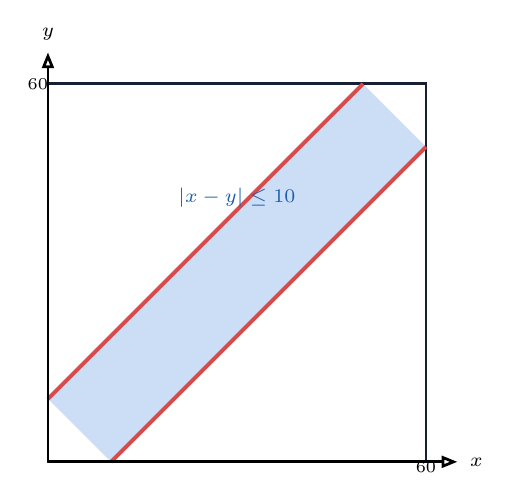
\begin{tikzpicture}[prob diagram,x=0.08cm,y=0.08cm]
    \draw[probInk,line width=1pt] (0,0) -- (0,60) -- (60,60) -- (60,0) -- cycle;
    \fill[probBlue,fill opacity=0.24]
      (0,10) -- (10,0) -- (60,50) -- (50,60) -- cycle;
    \draw[probRed,line width=1.4pt] (10,0) -- (60,50);
    \draw[probRed,line width=1.4pt] (0,10) -- (50,60);
    \draw[->] (0,0) -- (65,0);
    \draw[->] (0,0) -- (0,65);
    \node[anchor=west] at (67,0) {$x$};
    \node[anchor=south] at (0,67) {$y$};
    \node[anchor=north,font=\fontsize{6.5}{7.8}\selectfont] at (60,0) {60};
    \node[anchor=east,font=\fontsize{6.5}{7.8}\selectfont] at (0,60) {60};
    \node[text=probDarkBlue] at (30,42) {$|x-y|\leq 10$};
  \end{tikzpicture}%
}

% Source: prob-02-random-variables-diagram-01().
\expandafter\newcommand\csname prob-02-random-variables-diagram-01\endcsname{%
  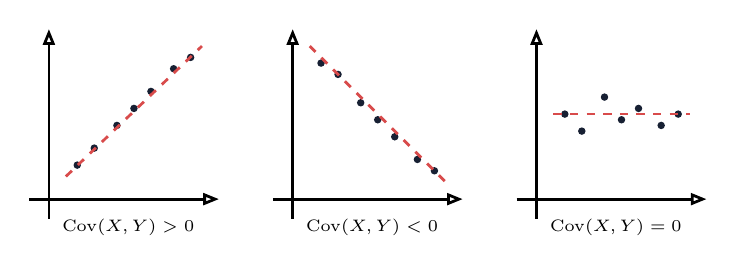
\begin{tikzpicture}[prob diagram,x=0.72cm,y=0.72cm]
    \ProbCovariancePanel{0}
      {0.5/0.6,0.8/0.9,1.2/1.3,1.5/1.6,1.8/1.9,2.2/2.3,2.5/2.5}
      {(0.3,0.4)}{(2.7,2.7)}{$\mathrm{Cov}(X,Y)>0$}
    \ProbCovariancePanel{4.3}
      {0.5/2.4,0.8/2.2,1.2/1.7,1.5/1.4,1.8/1.1,2.2/0.7,2.5/0.5}
      {(0.3,2.7)}{(2.7,0.3)}{$\mathrm{Cov}(X,Y)<0$}
    \ProbCovariancePanel{8.6}
      {0.5/1.5,0.8/1.2,1.2/1.8,1.5/1.4,1.8/1.6,2.2/1.3,2.5/1.5}
      {(0.3,1.5)}{(2.7,1.5)}{$\mathrm{Cov}(X,Y)=0$}
  \end{tikzpicture}%
}

% circular-dependence(): shared by the two original public diagram names.
\newcommand{\ProbCircularDependence}{%
  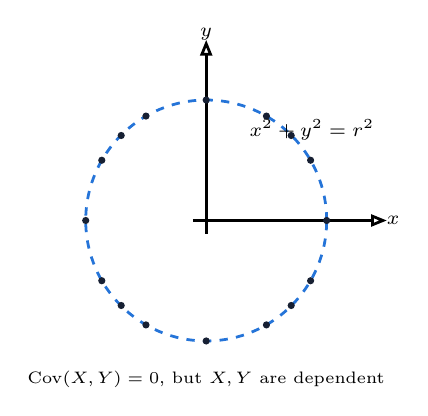
\begin{tikzpicture}[prob diagram,x=0.85cm,y=0.85cm]
    \ProbDiagramAxes{2.7}{2.7}{$x$}{$y$}
    \draw[probBlue,dashed] (0,0) circle[radius=1.8];
    \foreach \probX/\probY in {
      1.8/0,1.27/1.27,0/1.8,-1.27/1.27,
      -1.8/0,-1.27/-1.27,0/-1.8,1.27/-1.27,
      1.56/0.9,0.9/1.56,-0.9/1.56,-1.56/0.9,
      -1.56/-0.9,-0.9/-1.56,0.9/-1.56,1.56/-0.9
    } {
      \fill[probInk] (\probX,\probY) circle[radius=1.3pt];
    }
    \node[anchor=west] at (0.65,1.35) {$x^2+y^2=r^2$};
    \node[anchor=north,font=\fontsize{6.2}{7.44}\selectfont]
      at (0,-2.25) {$\mathrm{Cov}(X,Y)=0$, but $X,Y$ are dependent};
  \end{tikzpicture}%
}

% Source: prob-02-random-variables-diagram-02().
\expandafter\newcommand\csname prob-02-random-variables-diagram-02\endcsname{%
  \ProbCircularDependence
}

% Source: prob-02-random-variables-diagram-03(): Poisson probabilities, lambda=3.
\expandafter\newcommand\csname prob-02-random-variables-diagram-03\endcsname{%
  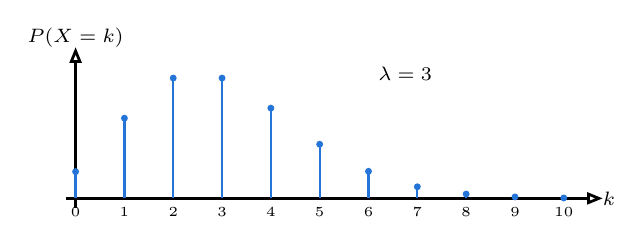
\begin{tikzpicture}[prob diagram,x=0.62cm,y=0.62cm]
    \ProbDiagramAxes{10.8}{3.1}{$k$}{$P(X=k)$}
    \foreach \probP [count=\probK from 0] in {
      0.04979,0.14936,0.22404,0.22404,0.16803,0.10082,
      0.05041,0.02160,0.00810,0.00270,0.00081
    } {
      \pgfmathsetmacro{\probHeight}{11*\probP}
      \draw[probBlue,line width=0.8pt] (\probK,0) -- (\probK,\probHeight);
      \fill[probBlue] (\probK,\probHeight) circle[radius=1.25pt];
      \node[anchor=north,font=\fontsize{5.5}{6.6}\selectfont]
        at (\probK,-0.18) {\probK};
    }
    \node[anchor=west] at (6.2,2.55) {$\lambda=3$};
  \end{tikzpicture}%
}

% Typst's f_X(x)/F_X(x) includes X(x) in the subscript. Preserve the source
% rendering here rather than silently changing that notation during conversion.
% Source: prob-02-random-variables-diagram-04(): uniform density.
\expandafter\newcommand\csname prob-02-random-variables-diagram-04\endcsname{%
  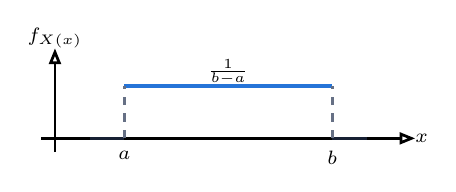
\begin{tikzpicture}[prob diagram,x=0.88cm,y=0.88cm]
    \ProbDiagramAxes{5.2}{1.3}{$x$}{$f_{X(x)}$}
    \draw[probInk,line width=1.2pt] (0.5,0) -- (1,0);
    \draw[prob curve] (1,0.75) -- (4,0.75);
    \draw[probInk,line width=1.2pt] (4,0) -- (4.5,0);
    \draw[prob guide] (1,0) -- (1,0.75);
    \draw[prob guide] (4,0) -- (4,0.75);
    \node[anchor=north] at (1,-0.18) {$a$};
    \node[anchor=north] at (4,-0.18) {$b$};
    \node at (2.5,0.95) {$\frac{1}{b-a}$};
  \end{tikzpicture}%
}

% Source: prob-02-random-variables-diagram-05(): uniform CDF.
\expandafter\newcommand\csname prob-02-random-variables-diagram-05\endcsname{%
  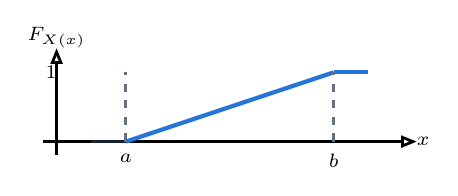
\begin{tikzpicture}[prob diagram,x=0.88cm,y=0.88cm]
    \ProbDiagramAxes{5.2}{1.35}{$x$}{$F_{X(x)}$}
    \draw[probInk,line width=1.2pt] (0.5,0) -- (1,0);
    \draw[prob curve] (1,0) -- (4,1);
    \draw[prob curve] (4,1) -- (4.5,1);
    \draw[prob guide] (1,0) -- (1,1);
    \draw[prob guide] (4,0) -- (4,1);
    \node[anchor=north] at (1,-0.18) {$a$};
    \node[anchor=north] at (4,-0.18) {$b$};
    \node[anchor=east] at (0,1) {$1$};
  \end{tikzpicture}%
}

% Source: prob-02-random-variables-diagram-06().
% Keep the source's plotted exp(-0.5*x) and its general density label verbatim.
\expandafter\newcommand\csname prob-02-random-variables-diagram-06\endcsname{%
  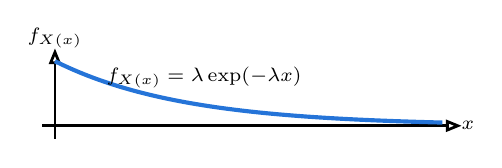
\begin{tikzpicture}[prob diagram,x=0.82cm,y=0.82cm]
    \ProbDiagramAxes{6.3}{1.2}{$x$}{$f_{X(x)}$}
    \draw[prob curve] plot[domain=0:6,samples=81] (\x,{exp(-0.5*\x)});
    \node[anchor=west] at (0.8,0.75) {$f_{X(x)}=\lambda\exp(-\lambda x)$};
  \end{tikzpicture}%
}

% Source: prob-02-random-variables-diagram-07(): exponential CDF.
\expandafter\newcommand\csname prob-02-random-variables-diagram-07\endcsname{%
  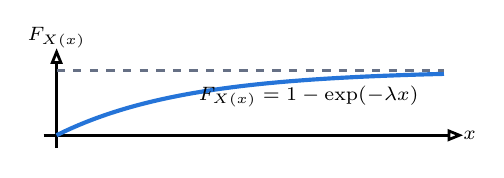
\begin{tikzpicture}[prob diagram,x=0.82cm,y=0.82cm]
    \ProbDiagramAxes{6.3}{1.35}{$x$}{$F_{X(x)}$}
    \draw[prob curve] plot[domain=0:6,samples=81] (\x,{1-exp(-0.5*\x)});
    \draw[prob guide] (0,1) -- (6,1);
    \node[anchor=west] at (2.2,0.6) {$F_{X(x)}=1-\exp(-\lambda x)$};
  \end{tikzpicture}%
}

% gamma-pdf/gamma-cdf(alpha,x): exact integer-shape formulae from Typst.
\pgfmathdeclarefunction{probGammaPdf}{2}{%
  \pgfmathparse{ifthenelse(#1==1,exp(-#2),
    ifthenelse(#1==2,#2*exp(-#2),
    ifthenelse(#1==3,#2*#2*exp(-#2)/2,
      #2*#2*#2*#2*exp(-#2)/24)))}%
}
\pgfmathdeclarefunction{probGammaCdf}{2}{%
  \pgfmathparse{ifthenelse(#1==1,1-exp(-#2),
    ifthenelse(#1==2,1-(1+#2)*exp(-#2),
    ifthenelse(#1==3,1-(1+#2+#2*#2/2)*exp(-#2),
      1-(1+#2+#2*#2/2+#2*#2*#2/6+#2*#2*#2*#2/24)*exp(-#2))))}%
}

% Source: prob-02-random-variables-diagram-08(): alpha=1,2,3,5; lambda=1.
\expandafter\newcommand\csname prob-02-random-variables-diagram-08\endcsname{%
  \begin{tikzpicture}[prob diagram,x=0.72cm,y=0.72cm]
    \ProbDiagramAxes{8.3}{1.2}{$x$}{$f_{X(x)}$}
    \foreach \probAlpha/\probColor in {1/probBlue,2/probRed,3/probGreen,5/probPurple} {
      \draw[\probColor,line width=1.25pt]
        plot[domain=0.05:8,samples=121] (\x,{probGammaPdf(\probAlpha,\x)});
    }
    \node[anchor=north] at (4.2,-0.35) {Gamma densities, $\lambda=1$};
  \end{tikzpicture}%
}

% Source: prob-02-random-variables-diagram-09(): alpha=1,2,3,5; lambda=1.
\expandafter\newcommand\csname prob-02-random-variables-diagram-09\endcsname{%
  \begin{tikzpicture}[prob diagram,x=0.72cm,y=0.72cm]
    \ProbDiagramAxes{8.3}{1.3}{$x$}{$F_{X(x)}$}
    \foreach \probAlpha/\probColor in {1/probBlue,2/probRed,3/probGreen,5/probPurple} {
      \draw[\probColor,line width=1.25pt]
        plot[domain=0:8,samples=121] (\x,{probGammaCdf(\probAlpha,\x)});
    }
    \draw[prob guide] (0,1) -- (8,1);
    \node[anchor=north] at (4.2,-0.35) {Gamma cdfs, $\lambda=1$};
  \end{tikzpicture}%
}

% Source: prob-03-joint-conditional-distribution-diagram-01().
\expandafter\newcommand\csname prob-03-joint-conditional-distribution-diagram-01\endcsname{%
  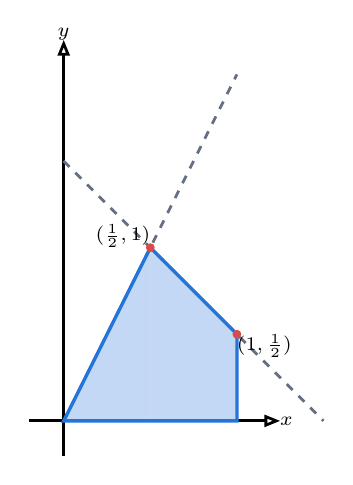
\begin{tikzpicture}[prob diagram,x=2.2cm,y=2.2cm]
    \ProbDiagramAxes{1.25}{2.2}{$x$}{$y$}
    \draw[prob guide] (0,0) -- (1,2);
    \draw[prob guide] (0,1.5) -- (1.5,0);
    \fill[probBlue,fill opacity=0.28] (0,0) -- (0.5,0) -- (0.5,1) -- cycle;
    \fill[probBlue,fill opacity=0.28]
      (0.5,0) -- (1,0) -- (1,0.5) -- (0.5,1) -- cycle;
    \draw[probBlue,line width=1.2pt]
      (0,0) -- (0.5,1) -- (1,0.5) -- (1,0) -- cycle;
    \fill[probRed] (0.5,1) circle[radius=1.6pt];
    \fill[probRed] (1,0.5) circle[radius=1.6pt];
    \node[anchor=south east] at (0.5,1) {$(\frac{1}{2},1)$};
    \node[anchor=north west] at (1,0.5) {$(1,\frac{1}{2})$};
  \end{tikzpicture}%
}

% Source: prob-03-joint-conditional-distribution-diagram-02().
\expandafter\newcommand\csname prob-03-joint-conditional-distribution-diagram-02\endcsname{%
  \ProbCircularDependence
}

% Source: prob-03-joint-conditional-distribution-diagram-03().
\expandafter\newcommand\csname prob-03-joint-conditional-distribution-diagram-03\endcsname{%
  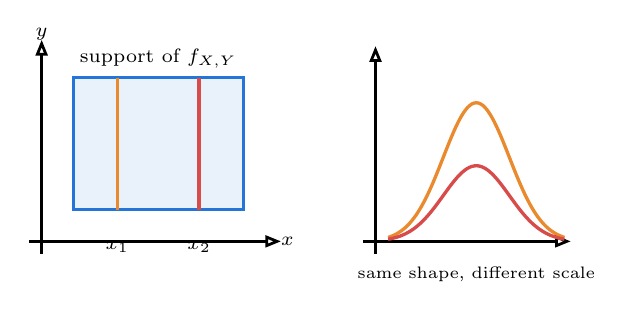
\begin{tikzpicture}[prob diagram,x=0.8cm,y=0.8cm]
    \ProbDiagramAxes{3.8}{3.2}{$x$}{$y$}
    \filldraw[fill=probBlue,fill opacity=0.1,draw=probBlue,
      draw opacity=1,line width=1pt]
      (0.5,0.5) -- (0.5,2.6) -- (3.2,2.6) -- (3.2,0.5) -- cycle;
    \draw[probOrange,line width=1.2pt] (1.2,0.5) -- (1.2,2.6);
    \draw[probRed,line width=1.2pt] (2.5,0.5) -- (2.5,2.6);
    \node[anchor=north] at (1.2,0) {$x_1$};
    \node[anchor=north] at (2.5,0) {$x_2$};
    \node at (1.85,2.9) {support of $f_{X,Y}$};
    \draw[->] (5.1,0) -- (8.4,0);
    \draw[->] (5.3,-0.2) -- (5.3,3.1);
    \draw[probOrange,line width=1.2pt]
      plot[domain=0.2:3,samples=81] ({5.3+\x},{2.2*exp(-((\x-1.6)*(\x-1.6))/0.55)});
    \draw[probRed,line width=1.2pt]
      plot[domain=0.2:3,samples=81] ({5.3+\x},{1.2*exp(-((\x-1.6)*(\x-1.6))/0.55)});
    \node[anchor=north,font=\fontsize{6.5}{7.8}\selectfont]
      at (6.9,-0.4) {same shape, different scale};
  \end{tikzpicture}%
}

% Source: prob-04-lln-diagram-01(): shaded right tail.
\expandafter\newcommand\csname prob-04-lln-diagram-01\endcsname{%
  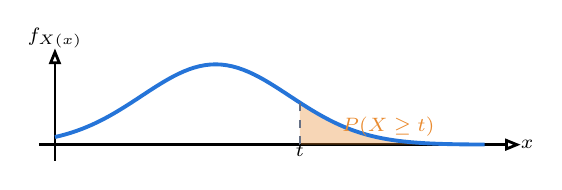
\begin{tikzpicture}[prob diagram,x=1.02cm,y=1.02cm]
    \ProbDiagramAxes{5.8}{1.2}{$x$}{$f_{X(x)}$}
    \fill[probOrange,fill opacity=0.35]
      (3.05,0) -- plot[domain=3.05:5.35,samples=81]
        (\x,{exp(-((\x-2)*(\x-2))/1.7)}) -- (5.35,0) -- cycle;
    \draw[probBlue,line width=1.4pt] plot[domain=0:5.35,samples=81]
      (\x,{exp(-((\x-2)*(\x-2))/1.7)});
    \draw[prob guide] (3.05,0) -- (3.05,{exp(-((3.05-2)*(3.05-2))/1.7)});
    \node[anchor=north] at (3.05,0) {$t$};
    \node[text=probOrange] at (4.15,0.22) {$P(X\geq t)$};
  \end{tikzpicture}%
}
\fi
